\documentclass[11pt, spanish]{memoir}
\usepackage[utf8]{inputenc}
\usepackage[spanish]{babel}
\usepackage{hyperref}
\usepackage{graphicx}
\usepackage{listings}
\usepackage{float}
\usepackage[T1]{fontenc}
\usepackage{kpfonts}
\setSingleSpace{1.1}
\SingleSpacing
\usepackage{xcolor,calc, blindtext}
\definecolor{chaptercolor}{gray}{0.8}
% helper macros
\newcommand\numlifter[1]{\raisebox{-2cm}[0pt][0pt]{\smash{#1}}}
\newcommand\numindent{\kern37pt}
\newlength\chaptertitleboxheight
\makechapterstyle{hansen}{
  \renewcommand\printchaptername{\raggedleft}
  \renewcommand\printchapternum{%
    \begingroup%
    \leavevmode%
    \chapnumfont%
    \strut%
    \numlifter{\thechapter}%
    \numindent%
\endgroup%
}
  \renewcommand*{\printchapternonum}{%
    \vphantom{\begingroup%
      \leavevmode%
      \chapnumfont%
      \numlifter{\vphantom{9}}%
      \numindent%
      \endgroup}
    \afterchapternum}
  \setlength\midchapskip{0pt}
  \setlength\beforechapskip{0.5\baselineskip}
  \setlength{\afterchapskip}{3\baselineskip}
  \renewcommand\chapnumfont{%
    \fontsize{4cm}{0cm}%
    \bfseries%
    \sffamily%
    \color{chaptercolor}%
  }
  \renewcommand\chaptitlefont{%
    \normalfont%
    \huge%
    \bfseries%
    \raggedleft%
  }%
  \settototalheight\chaptertitleboxheight{%
    \parbox{\textwidth}{\chaptitlefont \strut bg\\bg\strut}}
  \renewcommand\printchaptertitle[1]{%
    \parbox[t][\chaptertitleboxheight][t]{\textwidth}{%
      %\microtypesetup{protrusion=false}% add this if you use microtype
      \chaptitlefont\strut ##1\strut}%
}}
\chapterstyle{hansen}
\aliaspagestyle{chapter}{empty} % just to save some space
\begin{document}
\chapter{Instalación de MADMex}
Para instalar el sistema MADMex, es necesario contar con una instalación de GDAL
 funcionando correctamente. También es necesario contar con un interprete de Python
 y que el mismo se encuentre instalado en las variables de entorno, de modo que sea
 ejecutable desde una consola de comandos.
Se accede a la página localizada en:

\url{http://nodo2.conabio.gob.mx:8080/job/Madmex/}

\begin{figure}[H]
\centering
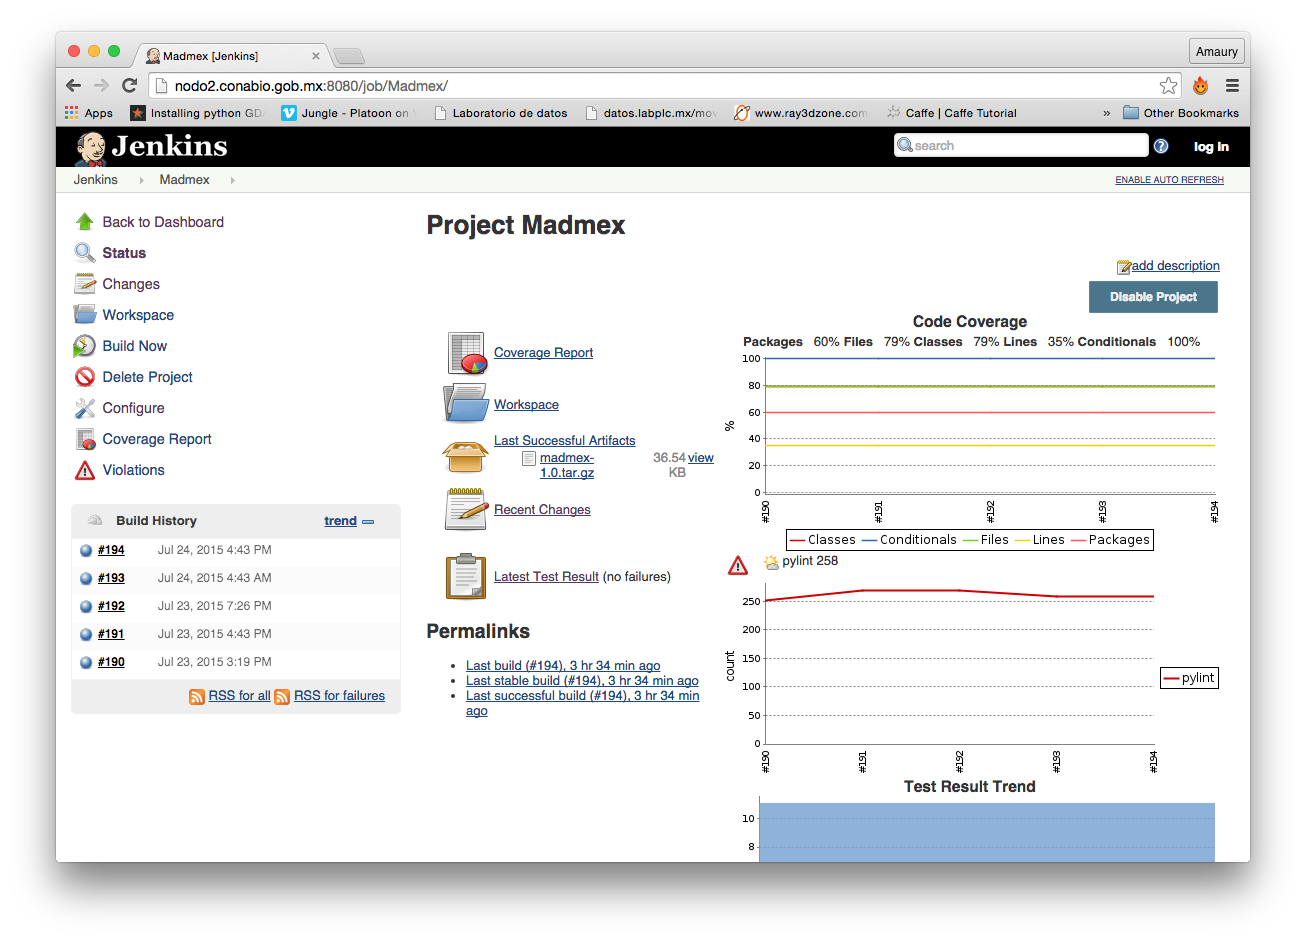
\includegraphics[width=14cm]{screen1.png}
\caption{Pantalla de descarga. \label{overflow}}
\end{figure}
Al hacer click en el link madmex-1.0.tar.gz se descargará un paquete que incluye
los archivos necesarios para instalar el sistema. Una vez que se cuenta con el
archivo tar, es necesario descomprimirlo (Un descompresor de archivos zip puede
hacerlo, uno open source se puede encontrar en \url{http://www.7-zip.org/}). La
instalación se realiza desde la consola. Para abrir la consola de comandos se puede
escribir cmd en el buscador del Inicio.

\begin{figure}[H]
\centering
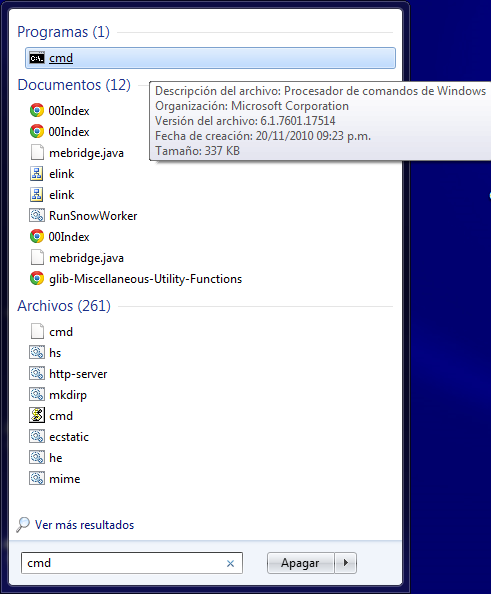
\includegraphics[width=6cm]{command1.png}
\caption{Pantalla de descarga. \label{overflow}}
\end{figure}

Navegando hasta la carpeta descomprimida
se introduce el siguiente comando:

\begin{figure}[H]
\centering
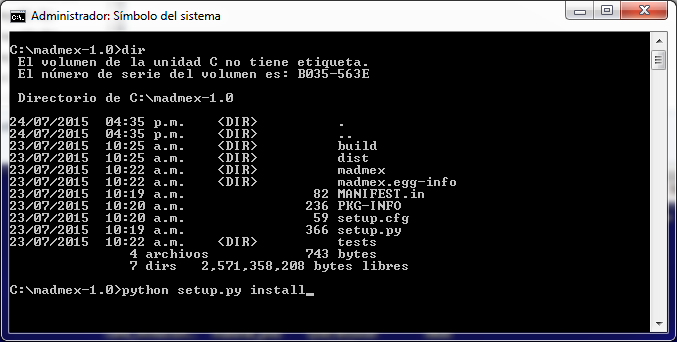
\includegraphics[width=14cm]{command2.png}
\caption{Pantalla de descarga. \label{overflow}}
\end{figure}
En caso de que el comando anterior funcione correctamente, la salida del sistema sera
 algo como:
\begin{figure}[H]
\centering
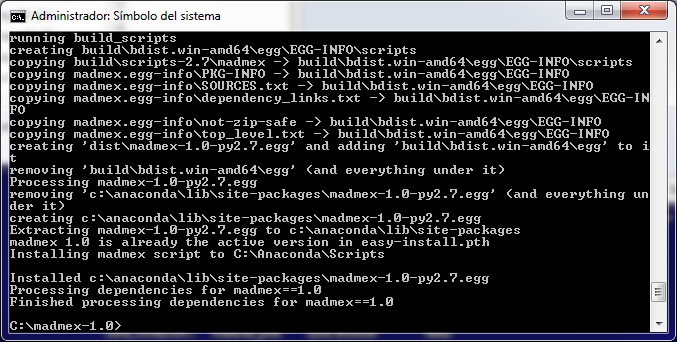
\includegraphics[width=14cm]{command3.png}
\caption{Pantalla de descarga. \label{overflow}}
\end{figure}

Por último para realizar el preprocesamiento de las imágenes se escribe el comando:

\begin{figure}[H]
\centering
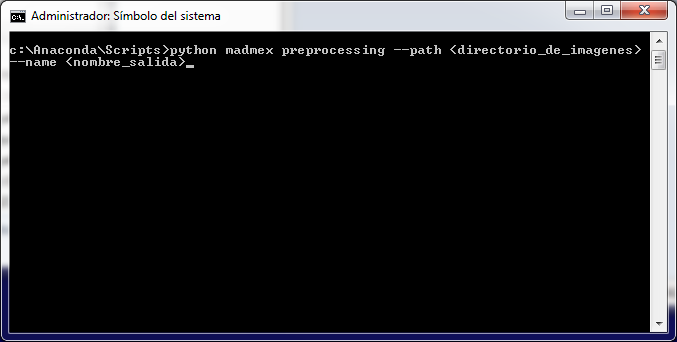
\includegraphics[width=14cm]{command4.png}
\caption{Pantalla de descarga. \label{overflow}}
\end{figure}


\end{document}
